%Version 3.1 December 2024
% See section 11 of the User Manual for version history
%
%%%%%%%%%%%%%%%%%%%%%%%%%%%%%%%%%%%%%%%%%%%%%%%%%%%%%%%%%%%%%%%%%%%%%%
%%                                                                 %%
%% Please do not use \input{...} to include other tex files.       %%
%% Submit your LaTeX manuscript as one .tex document.              %%
%%                                                                 %%
%% All additional figures and files should be attached             %%
%% separately and not embedded in the \TeX\ document itself.       %%
%%                                                                 %%
%%%%%%%%%%%%%%%%%%%%%%%%%%%%%%%%%%%%%%%%%%%%%%%%%%%%%%%%%%%%%%%%%%%%%

%%\documentclass[referee,sn-basic]{sn-jnl}% referee option is meant for double line spacing

%%=======================================================%%
%% to print line numbers in the margin use lineno option %%
%%=======================================================%%

%%\documentclass[lineno,pdflatex,sn-basic]{sn-jnl}% Basic Springer Nature Reference Style/Chemistry Reference Style

%%=========================================================================================%%
%% the documentclass is set to pdflatex as default. You can delete it if not appropriate.  %%
%%=========================================================================================%%

%%\documentclass[sn-basic]{sn-jnl}% Basic Springer Nature Reference Style/Chemistry Reference Style

%%Note: the following reference styles support Namedate and Numbered referencing. By default the style follows the most common style. To switch between the options you can add or remove “Numbered” in the optional parenthesis. 
%%The option is available for: sn-basic.bst, sn-chicago.bst%  
 
%%\documentclass[pdflatex,sn-nature]{sn-jnl}% Style for submissions to Nature Portfolio journals
%%\documentclass[pdflatex,sn-basic]{sn-jnl}% Basic Springer Nature Reference Style/Chemistry Reference Style
\documentclass[pdflatex,sn-mathphys-num]{sn-jnl}% Math and Physical Sciences Numbered Reference Style
%%\documentclass[pdflatex,sn-mathphys-ay]{sn-jnl}% Math and Physical Sciences Author Year Reference Style
%%\documentclass[pdflatex,sn-aps]{sn-jnl}% American Physical Society (APS) Reference Style
%%\documentclass[pdflatex,sn-vancouver-num]{sn-jnl}% Vancouver Numbered Reference Style
%%\documentclass[pdflatex,sn-vancouver-ay]{sn-jnl}% Vancouver Author Year Reference Style
%%\documentclass[pdflatex,sn-apa]{sn-jnl}% APA Reference Style
%%\documentclass[pdflatex,sn-chicago]{sn-jnl}% Chicago-based Humanities Reference Style

%%%% Standard Packages
%%<additional latex packages if required can be included here>

\usepackage{graphicx}%
\usepackage{multirow}%
\usepackage{amsmath,amssymb,amsfonts}%
\usepackage{amsthm}%
\usepackage{mathrsfs}%
\usepackage[title]{appendix}%
\usepackage{xcolor}%
\usepackage{textcomp}%
\usepackage{manyfoot}%
\usepackage{booktabs}%
\usepackage{algorithm}%
\usepackage{algorithmicx}%
\usepackage{algpseudocode}%
\usepackage{listings}%
\usepackage{tikz}
\usepackage{subcaption}
%%%%

%%%%%=============================================================================%%%%
%%%%  Remarks: This template is provided to aid authors with the preparation
%%%%  of original research articles intended for submission to journals published 
%%%%  by Springer Nature. The guidance has been prepared in partnership with 
%%%%  production teams to conform to Springer Nature technical requirements. 
%%%%  Editorial and presentation requirements differ among journal portfolios and 
%%%%  research disciplines. You may find sections in this template are irrelevant 
%%%%  to your work and are empowered to omit any such section if allowed by the 
%%%%  journal you intend to submit to. The submission guidelines and policies 
%%%%  of the journal take precedence. A detailed User Manual is available in the 
%%%%  template package for technical guidance.
%%%%%=============================================================================%%%%

%% as per the requirement new theorem styles can be included as shown below
\theoremstyle{thmstyleone}%
\newtheorem{theorem}{Theorem}%  meant for continuous numbers
\newtheorem{lemma}[theorem]{Lemma}%
\newtheorem{proposition}[theorem]{Proposition}% 
\newtheorem{corollary}[theorem]{Corollary}%
\newtheorem{example}[theorem]{Example}%
\newtheorem{remark}[theorem]{Remark}%
\newtheorem{definition}[theorem]{Definition}%
\newtheorem{problem}[theorem]{Problem}%
\newcommand{\len}[1]{\text{len}{(#1)}}

\raggedbottom
%%\unnumbered% uncomment this for unnumbered level heads

\begin{document}

\title[The minimum cost confluent flow problem and its extensions]{The minimum cost confluent flow problem and its extensions}

%%=============================================================%%
%% GivenName	-> \fnm{Joergen W.}
%% Particle	-> \spfx{van der} -> surname prefix
%% FamilyName	-> \sur{Ploeg}
%% Suffix	-> \sfx{IV}
%% \author*[1,2]{\fnm{Joergen W.} \spfx{van der} \sur{Ploeg} 
%%  \sfx{IV}}\email{iauthor@gmail.com}
%%=============================================================%%

\author*[1]{\fnm{Dag} \sur{Haugland}}\email{dag.haugland@ii.uib.no}
\author[2]{\fnm{Eligius M.T.} \sur{Hendrix}}\email{eligius@uma.es}
\equalcont{The authors contributed equally to this work.}
\affil*[1]{\orgdiv{Department of Informatics}, \orgname{University of Bergen}, \orgaddress{\city{Bergen}, \country{Norway}}}
\affil[2]{\orgdiv{Department of Computer Architecture}, \orgname{Universidad de M\'alaga}, \orgaddress{\city{M\'alaga}, \country{Spain}}}

\abstract{
Network flow problems tend to undergo a transition from tractable to computationally demanding when special conditions are imposed on the flow.
An example, introduced about two decades ago, is the requirement that all flow leaving a network node must be allocated to a unique arc.
Such a split-free flow is called confluent.
In the current work, several extensions of confluent flow are conceptualized and analyzed.
The dual concept where merging is disallowed at all nodes suggests itself.
This is extended further through a disjunctive combination at every node, where the flow has to either enter or leave along a unique arc.
Each of these flow conditions has a weak counterpart:
A flow is weakly confluent if all paths from any node in the flow graph terminate at a common sink.

The current work proves that even the weak version of any of these flow conditions renders the minimum cost flow problem NP-hard. Hardness is shown to persist even in restricted instances, such as bipartite digraphs with only two sinks.
For one of the flow conditions, single- and multi-commodity flow formulations are given,
accompanied by proofs of their correctness. Valid inequalities intended for cutting-plane approaches are given for both formulations.
}
\keywords{
network flow, complexity, integer programming, valid inequalities
}
\pacs[MSC Classification]{90B10, 90C11, 90C27, 90C57}

\maketitle


%-------------------------------------------------------------------------------
\section{Introduction} \label{intro}

Classic network flow models, like the \textsc{Minimum Cost Network Flow Problem} and the \textsc{Maximum Flow Problem},
enjoy favorable computational properties as well as a wide range of applications.
Imposing simple conditions on the flow pattern may, however,
transform a computationally tractable problem into a model of which only small instances can be solved in practical time.
\citet{chen2006merge} introduce the concept of a \emph{confluent flow}, which is a network flow where each node has at most one flow-carrying leaving arc.
They prove that requiring the flow to be confluent, i.e., disallowing splitting of the flow at any node, may render otherwise well-solved flow models NP-hard.

Settings in which confluent flow makes sense are numerous.
According to \citet{chen2006merge,chen2007confluent}, routing on the internet is a prominent example.
An immediate consequence of a flow being confluent is that all flow leaving a given node arrives at a unique sink,
which is consistent with destination-based internet routing.
Other examples include evacuation systems \citep{mamada2005evacuation}, where the flow of people must be directed along a unique passageway.
Further, the confluent-flow condition applies to distribution networks where the distribution units must be organized in such a way that
all outbound transportation follows a unique link.

Extensions of confluent flow are straightforward to imagine.
A condition dual to the no-splitting rule is prohibition of merging.
By symmetry, it is plausible that optimizing network flow under the constraints that every node receives flow along a unique entering arc,
is as computationally demanding as the case of confluent flow.
In transportation and logistics, the said restriction has relevance whenever inbound flow cannot be distributed over multiple entering links.

Several well-studied flow models relate to confluent flow and extensions thereof.
The \textsc{Single-source Unsplittable Flow Problem} (UFP) \citep{kleinberg1996unsplittable,dinitz99} asks for a unique path from a given source to each of a set of sinks.
A demand is associated with each sink, and flow must be assigned to the paths such that the demand is satisfied and arc capacities are respected.
As the flow paths constituting a UFP solution may intersect at one or more nodes, it does not hold in general that it is confluent.
However, the reverse implication applies, even in a multi-source extension of UFP: If a flow is confluent, then it follows a unique path between any source-sink pair.

Another related flow model is the \textsc{Disjoint Path Problem} (DPP) \citep{kolliopoulos2007unsplittable} in digraphs, in which pairs consisting of one source and one sink are given.
The problem is to find the largest subset of the pairs that can be joined by arc- or node-disjoint paths.
Feasible solutions are, in the node-disjoint version, necessarily confluent.
In contrast, two arc-disjoint paths may intersect at some node, in which case the solution is not confluent.
Conversely, a confluent flow does not necessarily induce a feasible solution to any of the two DPP variants.

In the current work, we conceptualize natural extensions of the confluent flow model.
Already indicated above, a flow involving no mixing of streams from different arcs entering any node is referred to as the \emph{influent} flow model.
That is, a flow is influent if the reverse of it is confluent. We also introduce weaker flow conditions related to confluent and influent flow, respectively.
A flow is said to be \emph{weakly confluent} if all the flow leaving a node arrives at a unique sink.
Obviously, if a flow is confluent in the strong sense, it is also confluent in the weak sense, whereas the reverse implication does not hold in general.
An analogous weak counterpart of influent flow is also introduced.
Weakly influent flow thus means that every node receives flow from at most one source, although the flow may be distributed across multiple entering arcs.

The weak fluency conditions are motivated, e.g., by logistics problems where each distribution unit is able to handle multiple routes along which the material
is leaving (entering) the unit, given that the entire flow is destined for (originates from) a single recipient (supplier).
Another interesting flow model emerges when the distribution network may be composed of a mix of nodes, some of which handle incoming flow from a single supplier, and the rest handle flow to a single recipient. In more abstract terms, the flow in a digraph is said to be \emph{weakly confluent-influent} if the arcs carrying positive flow induce a subgraph where all source-sink paths intersecting any given node share either a common source or a common sink.
The strong counterpart of this condition is that either the in-degree or the out-degree of any node in the subgraph is at most one.

The support of a confluent (influent) flow is a forest of arborescences rooted at distinct sinks (sources), with the flow directed towards (from) the root.
When the conditions are satisfied only weakly, the support still has one connected component for each sink (in the weakly confluent case).
However, there may be multiple paths connecting a node and a sink.
Disregarding arc directions, the support of a confluent-influent flow may be a connected graph, even if the condition applies in the strong sense.

Since confluent flow models were introduced to the scientific community by \citet{chen2006merge,chen2007confluent}, some attention to the topic has been given in the literature.
In their seminal article, \citet{chen2006merge} analyze the problem of minimizing congestion, defined as the largest flow/capacity ratio across arcs,
when the flow must be confluent and satisfy demand at all sinks.
Approximating the minimum congestion to within a factor 4/3 is proved to be NP-hard.
The follow-up work \citep{chen2007confluent} strengthens this result, and concludes that hardness persists if the approximation bound is relaxed to $1+\log_2{|T|}/2$,
where $T$ is the set of sinks in the graph.
The problem of minimizing the congestion over the set of confluent flow vectors is generalized by \citet{donovan2007degreeconstrained}.
They prove that the problem remains NP-hard if the flow condition is relaxed to \emph{bifurcated flow}, which means that at most two arcs leaving any node may carry flow.
This concept is further generalized to other bounds on the number of such arcs.

\citet{dressler2010confluent} study the \textsc{Maximum Confluent Flow Problem}, for which they give complexity and approximability results.
In particular, the problem is proved to be NP-hard even for directed trees, but solvable in pseudo-polynomial time for graph classes of bounded treewidth.
The authors later prove that the single-sink version of the problem is solvable in polynomial time if the digraph is outerplanar \citep{dressler2014polynomial}.
\citet{bhatia2008traffic} study the \textsc{Traffic Engineering Problem}, which takes as input a graph with node capacities, and asks for a set of arcs of minimum total cost to be added, such that a confluent flow exists.
The requirement is that the supply at all nodes be routed confluently to the unique sink.
Even when the input graph is a tree, approximation algorithms for this problem exist only if $P=NP$.
\citet{shepherd2017inapprox} prove that the the same is required for the maximum confluent flow in a node-capacitated digraph with a single sink to be approximated within a factor below $\mathcal{O}(\sqrt{|A|})$, where $A$ is the arc set.
The minimum congestion in this type of graphs is equally hard to approximate \cite{shepherd2017inapprox}. Under mild assumptions about node supply and capacities, however, algorithms with approximation ratio given by high-degree polynomials in the logarithm of the node cardinality are known \cite{shepherd2015poly}.

In the current letter, the following contributions are made: The extensions of confluent flow discussed above are conceptualized.
The complexity of the corresponding minimum cost flow problems is analyzed, and simple NP-hardness proofs are provided.
With special focus on the \textsc{Weakly Confluent-Influent Minimum Cost Flow Problem}, integer programming (single and multi-commodity flow) formulations are given and proved to be correct.
In the context of these formulations, a group of redundant valid inequalities is constructed.

The remainder of the letter is organized as follows:
Mathematical notation and definitions of flow problems subject to fluency constraints are provided in Sections \ref{sec:problem} and \ref{sec:conf}.
Complexity results are summarized in Section~\ref{sec:compl}.
In Section~\ref{sec:wciMILP}, integer programming formulations are derived, and their correctness is proved.
Valid inequalities for the models are analyzed in Section~\ref{sec:vi}. Section \ref{sec:conc} summarizes our findings.

%-----------------------------------------------------------------------
\section{Mathematical notation and problem formulations}\label{sec:problem}

Let $D=(N,A)$ be a directed acyclic graph,
where the node set $N=S\cup P\cup T$ consists of the disjoint subsets $S$ of \emph{sources}, $P$ of \emph{internal nodes}, and $T$ of \emph{sinks}.
The sets of upstream and downstream neighbors of node $i\in N$ are denoted
$N_i^-=\left\{j\in N:(j,i)\in A\right\}$ and $N_i^+=\left\{j\in N:(i,j)\in A\right\}$, respectively.
The set of sources from which there exists a path to node $i$ in $D$ is denoted $S_i$,
and $T_i$ is the set of sinks to which there is a path from $i$.
Without relevant loss of generality, it is assumed that $S_i\neq\emptyset\neq T_i$ for every $i\in N$
(with the conventions that $s\in S_s$ and $t\in T_t$),
and that $N_s^-=N_t^+=\emptyset$ for every $s\in S$ and $t\in T$.

Define the vectors of arc \emph{costs} $\boldsymbol{c}\in\mathbb{Q}^{A}$ and arc \emph{capacities} $\boldsymbol{h}\in\mathbb{Q}_+^{A}$.
In the \textsc{Minimum Cost Flow Problem} (mcFP), the flow leaving a source and the flow entering a sink are subject to upper and lower bounds, respectively.
Let $b_s$ denote the \emph{supply} at source $s\in S$, let $b_t$ be the \emph{demand} at sink $t\in T$,
and let $\boldsymbol{b}=\left(b_u\right)_{u\in S\cup T}$.

For a flow vector $\boldsymbol{f}\in\mathbb{R}_+^A$, $f_i^-=\sum_{j\in N_i^-}f_{ji}$ and $f_i^+=\sum_{j\in N_i^+}f_{ij}$ denote the entering flow and the leaving flow at node $i\in N$, respectively. The \emph{flow polytope} is the set
\[F(D,\boldsymbol{h},\boldsymbol{b}) = \left\{\boldsymbol{f}\in\mathbb{R}_+^A:\boldsymbol{f}\leq\boldsymbol{h}, f_s^+\leq b_s ~(s\in S), f_p^+=f_p^- ~(p\in P), f_t^-\geq b_t ~(t\in T)\right\}.\]
For any $\boldsymbol{f}\in F(D,\boldsymbol{h},\boldsymbol{b})$, let $D(\boldsymbol{f})=\left(N(\boldsymbol{f}), A(\boldsymbol{f})\right)$ denote the
\emph{support} of $\boldsymbol{f}$, i.e., the subgraph of $D$ where $A(\boldsymbol{f})\subseteq A$ consists of arcs $(i,j)\in A$ with $f_{ij}>0$, and $N(\boldsymbol{f})\subseteq N$ consists of nodes in $N$ with at least one incident arc in $A(\boldsymbol{f})$. For any node set $U\subseteq N$, let $U(\boldsymbol{f})=U\cap N(\boldsymbol{f})$.

%-----------------------------------------------------------------
\section{Confluent flow and extensions} \label{sec:conf}
In the current letter, the notion of a \emph{confluent} flow \cite{chen2006merge} is pursued and extended.
First, confluence in the reverse flow direction is considered. Second, in Section~\ref{sec:weak}, a relaxed version of confluent flow is introduced.
\begin{definition} \label{def:conf}
A flow $\boldsymbol{f}\in F(D,\boldsymbol{h},\boldsymbol{b})$ is said to be \emph{confluent} if $|N_i^+(\boldsymbol{f})|\leq 1$ at all nodes $i\in N(\boldsymbol{f})$.
% $f_{ij}>0$ for at most one $j\in N_i^+$.
\qed
\end{definition}

That is, confluence means that while flow streams are allowed to merge at any internal node, the flow has to leave along a unique arc.
Moreover, all flow leaving a source must be allocated to the same arc. At the sinks $t\in T$, the condition is satisfied by the assumption $N_t^+=\emptyset$.

\subsection{Reversing the confluent-flow condition} \label{sec:inf}
The inflow counterpart of confluent flow, where merging is not allowed at internal nodes and sinks, is defined analogously:
\begin{definition} \label{def:inf}
A flow $\boldsymbol{f}\in F(D,\boldsymbol{h},\boldsymbol{b})$ is said to be \emph{influent} if $|N_i^-(\boldsymbol{f})|\leq 1$ at all $i\in N(\boldsymbol{f})$.
% A flow $\boldsymbol{f}\in F(D,\boldsymbol{h})$ is said to be \emph{influent} if, at all nodes $i\in P\cup T$, $f_{ji}>0$ for at most one $j\in N_i^-$.
\qed
\end{definition}

By Definitions~\ref{def:conf}--\ref{def:inf}, confluent and influent flow are dual concepts, where the duality corresponds to arc reversals.
Combining the concepts disjunctively at each node introduces another fluency condition:
\begin{definition} \label{def:confinf}
A flow $\boldsymbol{f}\in F(D,\boldsymbol{h},\boldsymbol{b})$ is said to be \emph{confluent-influent} if
$\displaystyle{\min\left\{\left|N_i^-(\boldsymbol{f})\right|,\left|N_i^+(\boldsymbol{f})\right|\right\}\leq 1}$ at all $i\in N(\boldsymbol{f})$.
\qed
\end{definition}

Observe that by the assumption $N_s^-=\emptyset=N_t^+$ for all $s\in S$ and $t\in T$,
the condition in Definition~\ref{def:confinf} is satisfied at all sources and sinks.
Hence, in a bipartite digraph, where $P=\emptyset$, any feasible flow is confluent-influent.
In an arbitrary digraph, a flow that is either confluent or influent is necessarily confluent-influent, but the converse is not true.

The mcFP is extended by imposing any of the fluency conditions:
\begin{problem} \label{prob:conf}
The \textsc{Minimum Cost Confluent Flow Problem} (mcCFP):
Find a flow $\boldsymbol{f}\in F(D,\boldsymbol{h},\boldsymbol{b})$ satisfying Definition~\ref{def:conf} such that the cost $\boldsymbol{c}\cdot\boldsymbol{f}$ is minimized.
\qed
\end{problem}
\noindent
Analogously, in correspondence with Definitions~\ref{def:inf} and \ref{def:confinf}, respectively, the 
\textsc{Minimum Cost Influent Flow Problem} (mcIFP) and the \textsc{Minimum Cost Confluent-Influent Flow Problem} (mcCIFP) are defined.

\subsection{Weak fluency conditions} \label{sec:weak}

% Different digraphs may be equivalent from the perspective of the mcFP. Splitting any node into two new ones joined by an arc with sufficiently large capacity and zero cost, leads to an equivalent instance of the mcFP.
% In contrast, the operation largely alters an mcCIFP instance, since any flow in the modified network is confluent-influent. A concept that is more resilient to graph alterations is introduced next.

\begin{definition} \label{def:weakconfinf}
A flow $\boldsymbol{f}$ in $D$ is said to be \emph{weakly confluent} if, for all $i\in N(\boldsymbol{f})$,
$D(\boldsymbol{f})$ has paths from $i$ to at most one sink $t\in T$.
If $D(\boldsymbol{f})$ has paths to $i$ from at most one source $s\in S$, then $\boldsymbol{f}$ is said to be \emph{weakly influent}.
If at least one of the conditions holds at all $i\in N(\boldsymbol{f})$, then $\boldsymbol{f}$ is \emph{weakly confluent-influent}.
\qed
\end{definition}

The first two weak fluency conditions introduced in Definition~\ref{def:weakconfinf} are implied by their strong counterpart. Moreover, in bipartite graphs, weak confluence or influence implies the corresponding condition in the strong sense.
However, a confluent-influent flow is not necessarily weakly confluent-influent. A counterexample is depicted in Fig.~\ref{fig:strong}, while Fig.~\ref{fig:weak} shows a flow that is confluent-influent only in the weak sense.
If all paths in $D$ have length at most 2, i.e., if $N_p^-\subseteq S$ and $N_p^+\subseteq T$ for all $p\in P$, then any weakly confluent-influent flow is also confluent-influent, and vice versa.

\begin{figure}
\centering
\begin{subfigure}{0.48\textwidth}
\centering
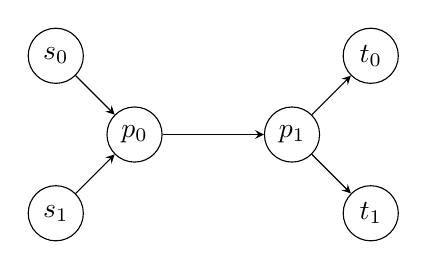
\begin{tikzpicture}[
    ->, 
    >=stealth,
    every node/.style={circle, draw, minimum size=7mm, inner sep=0pt}
]
    \node (1) at (0,2) {$s_0$};
    \node (2) at (0,0) {$s_1$};
    \node (3) at (1,1) {$p_0$};
    \node (4) at (3,1) {$p_1$};
    \node (5) at (4,2) {$t_0$};
    \node (6) at (4,0) {$t_1$};

    \draw (1) -- (3);
    \draw (2) -- (3);
    \draw (3) -- (4);
    \draw (4) -- (5);
    \draw (4) -- (6);
\end{tikzpicture}
 \subcaption{Strongly, not weakly, confluent-influent flow: At $p_0$ (at $p_1$), the flow is confluent (influent), but $p_0$ and $p_1$ receive flow from two sources and deliver to two sinks.} \label{fig:strong}
\end{subfigure}
\hfill
\begin{subfigure}{0.48\textwidth}
\centering
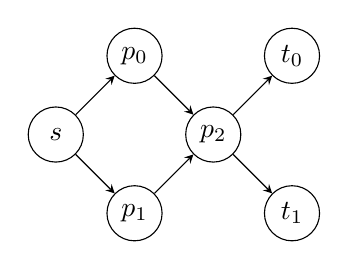
\begin{tikzpicture}[
    ->, 
    >=stealth,
    every node/.style={circle, draw, minimum size=7mm, inner sep=0pt}
]
    \node (1) at (0,1) {$s$};
    \node (2) at (1,2) {$p_0$};
    \node (3) at (1,0) {$p_1$};
    \node (4) at (2,1) {$p_2$};
    \node (5) at (3,2) {$t_0$};
    \node (6) at (3,0) {$t_1$};
    
    \draw (1) -- (2);
    \draw (1) -- (3);
    \draw (2) -- (4);
    \draw (3) -- (4);
    \draw (4) -- (5);
    \draw (4) -- (6);
\end{tikzpicture}
 \subcaption{Weakly, not strongly, confluent-influent flow: At $p_2$, the flow is neither confluent nor influent, but all nodes receive flow from a unique source.} \label{fig:weak}
\end{subfigure}
  \caption{Strongly and weakly confluent-influent flow}\label{fig:confinf}
\end{figure}


\section{Complexity of fluency-constrained extensions of mcFP} \label{sec:compl}
It is proved by \citet{chen2006merge} that a modified version of mcCFP, in which the congestion $\max_{(i,j)\in A}f_{ij}/h_{ij}$ is to be minimized, is NP-hard. Moreover, they show that it is NP-hard to approximate the minimum congestion within a factor $\tfrac{4}{3}$. In this section, similar results are given in the case of mcCFP and related problems.

\subsection{NP-hardness} \label{sec:nphard}
By a  reduction from the \textsc{Subset Sum Problem}, 
we show that mcCFP (Problem~\ref{prob:conf}) is NP-hard even in a restricted class of bipartite graphs.
\begin{proposition} \label{prop:conf}
For instances where $D$ is bipartite ($P=\emptyset$) and $|T|=2$, mcCFP is NP-hard.
\end{proposition}
\begin{proof}
We prove that checking whether $F(D,\boldsymbol{h},\boldsymbol{b})$ contains a confluent flow is NP-complete.

Consider an instance $(b_1,\ldots,b_n,d)$ of the \textsc{Subset Sum Problem}, with positive integers $1\leq b_1\leq\cdots\leq b_n\leq d$.
Let $D$ be the complete bipartite digraph with node sets $S=\{s_1,\ldots,s_n\}$ and $T=\{t_0,t_1\}$.
Let the supply at $s_i$ be $b_i$ ($i=1,\ldots,n$), while the demand at $t_0$ and $t_1$ is, respectively, $\sum_{i=1}^nb_i-d$ and $d$.
Both arcs leaving $s_i$ have capacity $b_i$.
Because total supply equals total demand, $\boldsymbol{f}\in F(D,\boldsymbol{h},\boldsymbol{b})$ if and only if $b_i$ flow units leave source $s_i$, $d$ units enter sink $t_1$, and $\sum_{i=1}^nb_i-d$ units enter sink $t_0$.
Confluence of $\boldsymbol{f}$ is thus equivalent to the condition that for all $i=1,\ldots,n$, $f_{s_it_k}=b_i$ and $f_{s_it_{1-k}}=0$ for some $k\in\{0,1\}$.
Hence, any confluent flow $\boldsymbol{f}\in F(D,\boldsymbol{h},\boldsymbol{b})$ satisfies $d=f_{t_1}^-=\sum_{s_i\in S_1}b_i$ for some $S_1\subseteq S$, which is precisely the condition for $(b_1,\ldots,b_n,d)$ to be a yes-instance of the \textsc{Subset Sum Problem}.
\end{proof}

NP-hardness in restricted instance classes also applies to the influent and confluent-influent counterparts of mcCFP.
In the influent case, the proof repeats the arguments in the proof of Proposition~\ref{prop:conf} applied to a digraph with all arcs reversed.
\begin{proposition} \label{prop:inf}
For instances where $D$ is bipartite ($P=\emptyset$) and $|S|=2$, mcIFP is NP-hard.
\end{proposition}
\begin{proof}
Consider the instance of the \textsc{Subset Sum Problem} introduced in the proof of Proposition~\ref{prop:conf}.
Let $D$ be a complete bipartite digraph with node sets $S=\{s_0,s_1\}$ and $T=\{t_1,\ldots,t_n\}$.
Let the demand at $t_i$ be $b_i$ ($i=1,\ldots,n$), while the supply at $s_0$ and $s_1$ is $\sum_{i=1}^nb_i-d$ and $d$, respectively.
Finally, $h_{st_i}=b_i$ for $s\in\{s_0,s_1\}$.
Following the arguments in the proof of Proposition~\ref{prop:conf}, there exists an influent flow $\boldsymbol{f}\in F(D,\boldsymbol{h},\boldsymbol{b})$
if and only if $\sum_{t_i\in T_1}b_i=d$ for some $T_1\subseteq T$.
\end{proof}

Proposition~\ref{prop:conf} also applies if mcCFP is defined with the demand as upper bounds
(if the constraints $f_t^-\geq b_t$ are replaced by $f_t^-\leq b_t$).
Consider the digraph introduced in the proof of the proposition, and let the cost $c_{st}=-2$ for all $s=s_1,\ldots,s_n$ and $t=t_1$.
For $t=t_0$, let $c_{st}=-1$.
Hence, the minimum cost is $-d-\sum_{i=1}^nb_i$ if and only if $\sum_{i\in S_1}b_i=d$ for some $S_1\subseteq\{1,\ldots,n\}$.
Analogously, Proposition~\ref{prop:inf} also holds if the definition of mcIFP undergoes a corresponding modification.

While mcCIFP is solvable in polynomial time in bipartite digraphs consisting only of sources and sinks,
introducing a set $P$ of intermediate nodes renders mcCIFP NP-hard, even if there are no arcs between any two nodes in $P$.
\begin{proposition} \label{prop:confinf}
mcCIFP is NP-hard in instances where $|T|=2$, $(N_p^-,N_p^+)=(S_p,T_p)$, and $\max\{|N_p^-|,|N_p^+|\}\leq 2$ for all $p\in P$.
\end{proposition}
\begin{proof}
Consider the instance $(b_1,\ldots,b_n,d)$ of the \textsc{Subset Sum Problem} introduced in the proof of Proposition~\ref{prop:conf}.
Let $D$ be the digraph with node sets $S=\{s_1,\ldots,s_n,s_1',\ldots,s_n'\}$, $P=\{p_1,\ldots,p_n\}$, and $T=\{t_0,t_1\}$.
Let all arcs of $D$ be incident to $P$, where $N_{p_i}^-=\{s_i,s_i'\}$ and  $N_{p_i}^+=\{t_0,t_1\}$.
Let the supply at $s_i$ and $s_i'$ be $b_i$ ($i=1,\ldots,n$), while the demand at $t_0$ and $t_1$ is, respectively, $2\sum_{i=1}^nb_i-2d$ and $2d$.
Both arcs entering $p_i$ have capacity $b_i$, whereas both the leaving arcs have capacity $2b_i$.

Consider a confluent-influent flow $\boldsymbol{f}\in F(D,\boldsymbol{h},\boldsymbol{b})$.
Since total supply equals both the total capacity of arcs leaving $S$ and total demand, it holds that $f_{sp_i}=h_{sp_i}=b_i>0$ for all $i=1,\ldots,n$ and $s\in\{s_i,s_i'\}$.
Because $\boldsymbol{f}$ is confluent-influent, and all $p_i\in P$ receive flow along two entering arcs,
all $2b_i$ units of flow leaving $p_i$ enter the same sink, $t_0$ or $t_1$.
Since $t_1$ receives $2d$ units of flow, there is a set $I_1\subseteq \{1,\ldots,n\}$ such that $f_{t_1}^-=\sum_{i\in I_1}f_{p_it_1}=2\sum_{i\in I_1}{b_i}=2d$,
and $(b_1,\ldots,b_n,d)$ is a yes-instance  of the \textsc{Subset Sum Problem}.

Conversely, if $\sum_{i\in I_1}b_i=d$ for some $I_1\subseteq\{1,\ldots,n\}$, then the flow $\boldsymbol{f}\in F(D,\boldsymbol{h},\boldsymbol{b})$, where $f_{s_ip_i}=f_{s_i'p_i}=b_i$ ($i=1,\ldots,n$),
$f_{p_it_0}=\left\{\begin{array}{lr}2b_i, & i\notin I_1 \\ 0, & i\in I_1,\end{array}\right.$ and
$f_{p_it_1}=\left\{\begin{array}{lr}2b_i, & i\in I_1 \\ 0, & i\notin I_1,\end{array}\right.$ is confluent-influent.
\end{proof}

\begin{corollary} \label{cor:nphard}
Checking feasibility of mcCFP, mcIFP, and mcCIFP is NP-hard.
\end{corollary}

Because Propositions~\ref{prop:conf}--\ref{prop:confinf} apply to instance classes in which the fluency condition in question is equivalent to its
weak counterpart, it follows immediately that the propositions apply even if the fluency condition is to be understood in the weak sense.

\subsection{Non-approximability} \label{sec:approx}
By Corollary~\ref{cor:nphard}, determining whether mcCFP is feasible is NP-hard in general. For instance classes where feasibility is guaranteed, the notion of approximation algorithms makes sense. We show next that such algorithms do not, in general, exist. 
This is true for all flow conditions under study, no matter if they apply weakly or strongly.

\begin{proposition} \label{prop:appr}
Consider the class of mcCFP instances in which there exist an arc set $A'\subseteq A$, where $|A'|=|T|$, such that $A'$ is a matching between $S$ and $T$, and $b_t\leq\min\{b_s,h_{st}\}$ for all $(s,t)\in A'$. There exists no approximation algorithm for this instance class, unless $P=NP$.
\end{proposition}
\begin{proof}
The proof is by contradiction. Assume $P\neq NP$ and that there exists an $\alpha>0$ and an algorithm that in polynomial time outputs a confluent flow with cost at most $(1+\alpha)$ times the minimum cost.
Consider the digraph defined in the proof of Proposition~\ref{prop:conf} extended by source nodes $\sigma_0$ and $\sigma_1$, and arcs $(\sigma_0,t_0)$ and $(\sigma_1,t_1)$.
Let the cost of the new arcs be $c_{\sigma_kt_k}=M+1$ ($k\in\{0,1\}$), where $M>\alpha$, and let all other arcs have cost $(\sum_{i=1}^nb_i)^{-1}$. Let the supply at $\sigma_0$ be $b_0=\sum_{i=1}^nb_i-d$, and let $h_{\sigma_0t_0}=b_0$ be the capacity of the arc leaving $\sigma_0$.
Likewise, let the supply at $\sigma_1$ and the capacity $h_{\sigma_1t1}$ of arc $(\sigma_1,t_1)$ be $d$.
Thus, the mcCFP instance belongs to the class in question, and is thereby feasible.
It follows that if the \textsc{Subset Sum} instance $(b_1,\ldots,b_n,d)$ is a yes-instance, then the mcCFP instance has minimum cost $z=1$.
Otherwise, $z\geq M+1>\alpha+1$.
Hence, the cost $z'$ of the confluent flow returned by the algorithm fulfills $z'\leq 1+\alpha$ if and only if $(b_1,\ldots,b_n,d)$ is a yes-instance, contradicting $P\neq NP$ and polynomiality of the algorithm.
\end{proof}

It is straightforward to see that Proposition~\ref{prop:appr} also applies to the weak mcCFP, and to the weak and strong variants of mcIFP and mcCIFP. Details on this are omitted.

\section{MILP formulations for weakly confluent-influent flow} \label{sec:wciMILP}

\subsection{Single-commodity flow formulations} \label{sec:sciMILP}
Combining single-commodity flow variables $\boldsymbol{f}$ with binary variables provides a natural formulation of the weak mcCIFP.
For all $p\in P$, we introduce binary variables $y_p^s$ for $s\in S_p$ and $y_p^t$ for $t\in T_p$. If $y_p^s=1$, then all paths from $S$ to $p$ in $D(\boldsymbol{f})$ are forced to start at $s$.
Analogously, $y_p^t=1$ implies that all paths from $p$ to $T$ terminate at $t$. The reverse implications do not hold in general: If $s$ and $t$ are the unique source and sink, respectively, to which node $p$ is connected in $D(\boldsymbol{f})$, then $(y_p^s,y_p^t)=(1,0)$ or $(y_p^s,y_p^t)=(0,1)$. Such ties are solved arbitrarily.
For notational convenience, we also define binary constants\\ $y_u^v=\left\{\begin{array}{lr}1, & u=v \\ 0, & u\neq v\end{array}\right.$
for all $u,v\in S\cup T$, and $y_p^u=0$ for all $p\in P$ and $u\in (S\setminus S_p)\cup(T\setminus T_p)$.

Following these definitions, a weakly confluent-influent flow fulfills for each intermediate node $p\in P$ the equality $\sum_{s\in S_p}y_p^s+\sum_{t\in T_p}y_p^t=1$.
Consistency between $\boldsymbol{f}$ and $\boldsymbol{y}=\left(y_p^u\right)_{p\in P, u\in S_p\cup T_p}$ implies that for all arcs $(i,j)\in A(\boldsymbol{f})$ and all $s\in S_j$, it holds that $y_i^s=1$ (node $i$ receives flow only from source $s$) if $y_j^s=1$ (node $j$ receives flow only from source $s$). Hence, $f_{ij}=0$ if $y_i^s=0$ and $y_j^s=1$. This relation is imposed by the inequality $f_{ij}\leq h_{ij}\left(1-y_j^s+y_i^s\right)$.
A symmetric argument suggests the constraint $f_{ij}\leq h_{ij}\left(1-y_i^t+y_j^t\right)$ for each $t\in T_i$.
An MILP model capturing the weakly confluent-influent property thus reads:
\begin{eqnarray}
\min & \sum_{(i,j)\in A}c_{ij}f_{ij} \label{eq:objMCCIFP} \\
     & \sum_{s\in S_p}y_p^s+\sum_{t\in T_p}y_p^t = 1 & p\in P \label{eq:convMCCIFP} \\
     & f_{ij}\leq h_{ij}\left(1-y_j^s+y_i^s\right) & (i,j)\in A, s\in S_j \label{eq:sMCCIFP} \\
     & f_{ij}\leq h_{ij}\left(1-y_i^t+y_j^t\right) & (i,j)\in A, t\in T_i \label{eq:tMCCIFP} \\
     & \boldsymbol{f}\in F(D,\boldsymbol{h},\boldsymbol{b}) \label{eq:fMCCIFP} \\
     & y_p^u\in\{0,1\} & p\in P, u\in S_p\cup T_p \label{eq:xMCCIFP}.
\end{eqnarray}

For arcs $(i,j)\in A$, where $i\in S$, \eqref{eq:sMCCIFP} is simplified to $f_{ij}\leq h_{ij}(1-y_j^s)$ for all $s\in S_j\setminus\{i\}$, since $y_i^s=0$.
Hence, arc $(i,j)$ does not carry flow if $y_j^s=1$, which means that $j$ receives all its flow from some source $s\neq i$.
Likewise, \eqref{eq:tMCCIFP} implies zero flow along arc $(i,j)$ if $j\in T$ and $y_i^t=1$ for some sink $t\in T_i\setminus\{j\}$.

If $i\in P$ and $s\in S_j\setminus S_i$, i.e., if $D$ has a path from source $s$ to node $j$ but not to node $i$, then $y_i^s=0$.
From \eqref{eq:sMCCIFP}, it follows that if $y_j^s=1$, then $f_{ij}=0$.

The correspondence of the feasible region of model \eqref{eq:objMCCIFP}--\eqref{eq:xMCCIFP} with the  weakly confluent-influent flows in $F(D,\boldsymbol{h},\boldsymbol{b})$ is given by the following lemma. 
\begin{lemma} \label{lem:MCCIFP}
Let $(\boldsymbol{f},\boldsymbol{y})$ be a feasible solution to \eqref{eq:objMCCIFP}--\eqref{eq:xMCCIFP}.
For every path $(s,p_1,\ldots,p_r,t)$ in $D(\boldsymbol{f})$, where $s\in S$ and $t\in T$,
there exists some integer $q\in\{0,1,\ldots,r\}$ such that $y_{p_k}^s=1$ for all $0\leq k\leq q$ and $y_{p_k}^t=1$ for all $q<k\leq r+1$, where $p_0=s$ and $p_{r+1}=t$.
\end{lemma}
\begin{proof}
Consider any $k\in\{0,1,\ldots,r+1\}$.
By \eqref{eq:convMCCIFP} and \eqref{eq:xMCCIFP}, $y_{p_k}^{u_k}=1$ for a unique $u_k\in S\cup T$, where $u_0=s$ and $u_{r+1}=t$.
Let $q=\max\{k=0,1,\ldots,r: u_k\in S\}$.
If $q=0$, $u_q=s$ immediately follows.
Otherwise, \eqref{eq:sMCCIFP} applied to $(i,j)=(p_{q-1},p_q)\in A$ yields $y_{p_{q-1}}^{u_q}=1$, since $(p_{k-1},p_k)\in A(\boldsymbol{f})$ implies $f_{p_{k-1}p_k}>0$.
By induction, it follows that $y_{p_k}^{u_q}=1$ for $k=q,q-1,\ldots,0$, and $y_{p_0}^{u_q}=y_s^{u_q}=1$ yields $u_q=s$.
Hence, $y_{p_0}^s=\cdots=y_{p_q}^s=1$.

Analogously, since $u_{q+1}\in T$, \eqref{eq:tMCCIFP} applied to $(p_q,p_{q+1}),\ldots,(p_r,p_{r+1})$ yields $y_{p_k}^{u_{q+1}}=1$ for $k=q+1,\ldots,r+1$.
The observation that $y_{p_{r+1}}^{u_{q+1}}=y_{t}^{u_{q+1}}=1$ implies $u_{q+1}=t$ completes the proof.
\end{proof}

\begin{proposition} \label{prop:MCCIFP}
A vector $\boldsymbol{f}\in\mathbb{R}^A$ is a weakly confluent-influent flow in $F(D,\boldsymbol{h},\boldsymbol{b})$ if and only if there exists a binary vector $\boldsymbol{y}\in\{0,1\}^P$ such that $(\boldsymbol{f},\boldsymbol{y})$ satisfies \eqref{eq:convMCCIFP}--\eqref{eq:xMCCIFP}.
\end{proposition}
\begin{proof}
If: Assume $(\boldsymbol{f},\boldsymbol{y})$ satisfies \eqref{eq:convMCCIFP}--\eqref{eq:xMCCIFP}.
Consider an arbitrary $p\in P(\boldsymbol{f})$.
If $y_p^s=1$ for some $s\in S$, Lemma~\ref{lem:MCCIFP} says that $y_u^s=1$ at all nodes $u$ on paths from $S$ to $p$ in $D(\boldsymbol{f})$.
Since $y_u^s=0$ at sources $u\neq s$, it follows that all paths to $p$ start at source $s$.
Otherwise, $y_p^t=1$ for some $t\in T$. By Lemma~\ref{lem:MCCIFP}, $y_u^t=1$ at all nodes $u$ on paths from $p$ to $T$, and $y_u^t=0$ at sinks $u\neq t$ proves that all paths terminate at sink $t$.
Hence, $\boldsymbol{f}$ is a weakly confluent-influent flow in $F(D,\boldsymbol{h},\boldsymbol{b})$.

Only if: Assume $\boldsymbol{f}$ is a weakly confluent-influent flow, which immediately implies \eqref{eq:fMCCIFP}.
For all $p\in P\setminus P(\boldsymbol{f})$ and $u\in S_p\cup T_p$, choose $y_p^u\in\{0,1\}$ arbitrarily such that \eqref{eq:convMCCIFP} is satisfied.
For arcs $(i,j)\in A\setminus A(\boldsymbol{f})$, $f_{ij}=0$ shows that \eqref{eq:sMCCIFP}--\eqref{eq:tMCCIFP} are satisfied.
Consider a $p\in P(\boldsymbol{f})$. If $p$ receives all its flow from a unique source $s$, let $y_p^s=1$ and $y_p^u=0$ for all $u\in T_p\cup S_p\setminus\{s\}$.
Otherwise, $p$ sends all flow to a unique sink $t$ since $\boldsymbol{f}$ is weakly confluent-influent.
In that case, let $y_p^t=1$ and $y_p^u=0$ for all $u\in S_p\cup T_p\setminus\{t\}$. Thus, \eqref{eq:convMCCIFP} is satisfied.
For any $(i,j)\in A(\boldsymbol{f})$, node $i$ receives all its flow from $s$ if node $j$ does.
Hence, $y_i^s=1$ if $y_j^s=1$. Analogously, $y_j^t=1$ if $y_i^t=1$.
Consequently, the right-hand side of \eqref{eq:sMCCIFP}--\eqref{eq:tMCCIFP} is no less than $h_{ij}$,
and the inequalities hold since $f_{ij}\leq h_{ij}$.
\end{proof}

\begin{corollary} \label{cor:MCCIFP}
For any feasible solution $(\boldsymbol{f},\boldsymbol{y})$ to \eqref{eq:objMCCIFP}--\eqref{eq:xMCCIFP},
the arc set \[\bar{A}(\boldsymbol{f})=\left\{(i,j)\in A(\boldsymbol{f}):\sum_{s\in S_i}y_i^s=\sum_{t\in T_j}y_j^t=1\right\}\] is a minimal cut in $D(\boldsymbol{f})$ separating $S$ from $T$.
\end{corollary}
\begin{proof}
Consider any $S$-$T$-path in $D(\boldsymbol{f})$.
The claim that $\bar{A}(\boldsymbol{f})$ is a cut follows by observing that according to Lemma~\ref{lem:MCCIFP}, there exists an arc $(i,j)$ on the path such that $y_i^s=y_j^t=1$ for some $(s,t)\in(S_i\times T_j)$.
To prove minimality, consider an arc $(i,j)\in\bar{A}(\boldsymbol{f})$, where $y_i^s=y_j^t=1$ for some $(s,t)\in S_i\times T_j$. Conservation of flow \eqref{eq:fMCCIFP} implies that $D(\boldsymbol{f})$ has paths from $S$ to $i$ and from $j$ to $T$. Thus, $\bar{A}(\boldsymbol{f})\setminus\{(i,j)\}$ is not a cut. 
\end{proof}

\subsection{Multi-commodity flow formulations} \label{sec:mciMILP}
For all $(i,j)\in A$ and $(s,t)\in S_i\times T_j$, let $x_{ij}^{st}$ denote the flow from source $s$ along arc $(i,j)$ to sink $t$,
and let $x_{ij}^{st}=0$ for $(s,t)\in (S\times T)\setminus(S_i\times T_j)$.
An upper bound, $h_{ij}^{st}\leq h_{ij}$, on this flow is given as the maximum flow from $j$ to $i$ in the digraph $D_{ij}^{st}=(N,A_{ij}^{st})$, where $A_{ij}^{st}=\left(A\cup\{(t,s)\}\right)\setminus\{(i,j)\}$ with capacity $h_{ts}=h_{ij}$ on arc $(t,s)$.
Let $\boldsymbol{x}^{st}=\left(x_{ij}^{st}\right)_{(i,j)\in A}$.

Recall the binary variables and constants $y_i^u$ ($i\in N$, $u\in S\cup T$) introduced in Section~\ref{sec:sciMILP},
along with the binary constants $y_u^v=1$ for $u=v$ and $y_u^v=0$ for $u\neq v$ ($u,v\in S\cup T$).
When transforming from single-commodity to multi-commodity flow variables, the proportion of the flow at node $p$ supplied from source $s$ and delivered to sink $t$ becomes useful.
For any $\boldsymbol{f}\in F(D,\boldsymbol{h},\boldsymbol{b})$, let $w_u^v=y_u^v$ for all $u,v\in S\cup T$, and let
\begin{eqnarray}
w_p^s = \frac{\sum_{i\in N_p^-}w_i^sf_{ip}}{\sum_{i\in N_p^-}f_{ip}}, & ~p\in P(\boldsymbol{f}), s\in S_p \label{eq:ws} \\
w_p^t = \frac{\sum_{j\in N_p^+}w_j^tf_{pj}}{\sum_{j\in N_p^+}f_{pj}}, & ~p\in P(\boldsymbol{f}), t\in T_p. \label{eq:wt}
\end{eqnarray}

\begin{lemma} \label{lem:w}
For all $p\in N(\boldsymbol{f})$, $\sum_{s\in S_p}w_p^s=\sum_{t\in T_p}w_p^t=1$.
\end{lemma}
\begin{proof}
For $i\in S$, $\sum_{s\in S}w_i^s=1$ is obvious. 
Assume $\sum_{s\in S_i}w_i^s=1$ for all $i\in N_p^-(\boldsymbol{f})$, where $p\in P(\boldsymbol{f})$.
Then, by \eqref{eq:ws}, $\sum_{s\in S_p}w_p^s=\sum_{s\in S_p}\frac{\sum_{i\in N_p^-}w_i^sf_{ip}}{\sum_{i\in N_p^-}f_{ip}}=1$.
Because $D(\boldsymbol{f})$ is acyclic, induction proves $\sum_{s\in S_p}w_p^s=1$ for all $p\in N(\boldsymbol{f})$.
The proof of $\sum_{t\in T_p}w_p^t=1$ is analogous.
\end{proof}

\begin{proposition} \label{prop:multi}
Let $(\boldsymbol{f},\boldsymbol{y})$ be a pair of vectors satisfying \eqref{eq:convMCCIFP} and \eqref{eq:fMCCIFP}--\eqref{eq:xMCCIFP}.
Then, inequalities \eqref{eq:sMCCIFP}--\eqref{eq:tMCCIFP} hold if and only if there exist flow vectors
$\boldsymbol{x}^{st}\in\mathbb{R}_+^A$ for all $(s,t)\in S\times T$ such that $\boldsymbol{f} = \sum_{(s,t)\in S\times T}\boldsymbol{x}^{st}$,
$\sum_{j\in N_i^-}x_{ji}^{st} = \sum_{j\in N_i^+}x_{ij}^{st}$ for all $i\in N(\boldsymbol{f})\setminus\{s,t\}$, and such that
$y_i^s+y_i^t=y_j^s+y_j^t=1\leq y_i^s+y_j^t$ for all $(i,j)\in A(\boldsymbol{x}^{st})$.
\end{proposition}
\begin{proof}
If: Assume that flow vectors $\boldsymbol{x}^{st}$ satisfying the said conditions exist.
At arcs $(i,j)\notin A(\boldsymbol{f})$, it holds that $f_{ij}=0$ satisfies \eqref{eq:sMCCIFP}--\eqref{eq:tMCCIFP} since the right-hand side of both inequalities is non-negative for all $(s,t)\in S_j\times T_i$.
For arcs $(i,j)\in A(\boldsymbol{f})$, observe first that \eqref{eq:fMCCIFP} implies $f_{ij}\leq h_{ij}$.
 Consider $v_{ij}^u=1-y_j^u+y_i^u$ if $u\in S_j$ and $v_{ij}^u=1-y_i^u+y_j^u$ if $u\in T_i$. It is sufficient to prove $v_{ij}^u\geq 1$ for all $u\in S_j\cup T_i$.
From $\boldsymbol{f} = \sum_{(s,t)\in S\times T}\boldsymbol{x}^{st}$, it follows that $(i,j)\in A(\boldsymbol{x}^{st})$ for at least one $(s,t)\in S_j\times T_i$.
Because of the assumption $y_i^s+y_i^t=y_j^s+y_j^t=1$, \eqref{eq:convMCCIFP} implies $y_i^u=y_j^u=0$ for all $u\in(S_j\cup T_i)\setminus\{s,t\}$, implying $v_{ij}^u=1$.
Further, combining \eqref{eq:convMCCIFP} and the assumption $y_i^s+y_j^t\geq 1$ yields $v_{ij}^s=1-y_j^s+y_i^s\geq y_j^t+y_i^s\geq 1$ and $v_{ij}^t=1-y_i^t+y_j^t\geq y_i^s+y_j^t\geq 1$. 
It follows that \eqref{eq:sMCCIFP}--\eqref{eq:tMCCIFP} hold for all $u\in S_j\cup T_i$.

Only if: 
Assume that $(\boldsymbol{f},\boldsymbol{y})$ satisfies \eqref{eq:sMCCIFP}--\eqref{eq:tMCCIFP}.
For arcs $(i,j)\in A(\boldsymbol{f})$, define $x_{ij}^{st} = f_{ij}w_i^sw_j^t$ for all $(s,t)\in S_i\times T_j$ and $x_{ij}^{st}=0$ for all $(s,t)\in(S\times T)\setminus(S_i\times T_j)$.
Let $x_{ij}^{st}=0$ for $(i,j)\in A\setminus A(\boldsymbol{f})$.
Utilizing \eqref{eq:ws}, conservation of flow, and \eqref{eq:wt} yields $\sum_{i\in N_p^-}x_{ip}^{st} = w_p^t\sum_{i\in N_p^-}w_i^sf_{ip} = w_p^tw_p^s\sum_{i\in N_p^-}f_{ip} = w_p^tw_p^s\sum_{j\in N_p^+}f_{pj} = w_p^s\sum_{j\in N_p^+}w_j^tf_{pj} = \sum_{j\in N_p^+}x_{pj}^{st}$.
Further, $\sum_{s\in S_i}\sum_{t\in T_j}x_{ij}^{st}=\sum_{s\in S_i}\sum_{t\in T_j}f_{ij}w_i^sw_j^t=f_{ij}$ by Lemma~\ref{lem:w}.

Consider any $(i,j)\in A$ and $(s,t)\in S_i\times T_j$ such that $(i,j)\in A(\boldsymbol{x}^{st})\subseteq A(\boldsymbol{f})$.
Since $\boldsymbol{x}^{st}$ satisfies conservation of flow at $P$, there exists a path in $D(\boldsymbol{x}^{st})$ from $s$ to $t$ intersecting $(i,j)$.
Because $\boldsymbol{x}^{st}\leq\boldsymbol{f}$, this is also a path in $D(\boldsymbol{f})$.
Lemma~\ref{lem:MCCIFP} then shows that for $k\in\{i,j\}$, either $y_k^s=1$ or $y_k^t=1$,
and that $y_i^s+y_j^t\geq 1$.
\end{proof}
\noindent
Proposition~\ref{prop:multi} suggests a multi-commodity flow formulation of the weak mcCIFP:

\begin{eqnarray}
\min & \sum_{(i,j)\in A}c_{ij}f_{ij} \label{eq:objmMCCIFP} \\
     & f_{ij} = \sum_{s\in S_i}\sum_{t\in T_j}x_{ij}^{st}, & (i,j)\in A \label{eq:fmMCCIFP} \\
     & \sum_{j\in N_i^-}x_{ji}^{st} = \sum_{j\in N_i^+}x_{ij}^{st}, & i\in P, s\in S_i, t\in T_i \label{eq:stmMCCIFP} \\
     & 0\leq x_{ij}^{st}\leq h_{ij}^{st}\left(y_k^s+y_k^t\right), & (i,j)\in A, s\in S_i, t\in T_j, k\in\{i,j\} \label{eq:istmMCCIFP} \\
%     & 0\leq x_{ij}^{st}\leq h_{ij}^{st}\left(y_j^s+y_j^t\right), & (i,j)\in A, s\in S_i, t\in T_j \label{eq:jtsmMCCIFP} \\
     & 0\leq x_{ij}^{st}\leq h_{ij}^{st}\left(y_i^s+y_j^t\right), & (i,j)\in A, s\in S_i, t\in T_j \label{eq:isjtmMCCIFP} \\
     & \eqref{eq:convMCCIFP}-\eqref{eq:xMCCIFP} \label{eq:allMCCIFP}
\end{eqnarray}

According to Proposition~\ref{prop:multi}, inequalities \eqref{eq:sMCCIFP}--\eqref{eq:tMCCIFP} are redundant in the multi-commodity formulation \eqref{eq:objmMCCIFP}--\eqref{eq:allMCCIFP}.
In the interest of a strong continuous relaxation, however, the constraints are included.

\subsection{Source-indexed flow commodities} \label{sec:mciMILPsource}

Model \eqref{eq:objmMCCIFP}--\eqref{eq:allMCCIFP} considers a flow commodity for each pair $(s,t)\in S\times T$. In a related model, the commodities correspond uniquely to the sources. Consider the flow variables $x_{ij}^s$ for each arc $(i,j)\in A$ and each source $s\in S_i$. A model analogous to \eqref{eq:objmMCCIFP}--\eqref{eq:allMCCIFP} is thus achieved by replacing \eqref{eq:fmMCCIFP}--\eqref{eq:stmMCCIFP} by 

\begin{eqnarray}
     & f_{ij} = \sum_{s\in S_i}x_{ij}^s, & (i,j)\in A \label{eq:fmsMCCIFP} \\
     & \sum_{j\in N_i^-}x_{ji}^s = \sum_{j\in N_i^+}x_{ij}^s, & i\in P, s\in S_i, \label{eq:smMCCIFP}
\end{eqnarray}
and \eqref{eq:istmMCCIFP}--\eqref{eq:isjtmMCCIFP} by 
\begin{eqnarray}
     & 0\leq x_{ij}^s\leq h_{ij}^s\left(y_i^s+\sum_{t\in T_j}y_i^t\right), & (i,j)\in A, s\in S_i, \label{eq:istmsMCCIFP}
\end{eqnarray}
\noindent
where $h_{ij}^s\leq h_{ij}$ is an upper bound on the flow along $(i,j)$ from $s$ to $T$.

That the model constituted by \eqref{eq:objmMCCIFP}, \eqref{eq:allMCCIFP}, and \eqref{eq:fmsMCCIFP}--\eqref{eq:istmsMCCIFP} is a valid formulation of the weak mcCIFP is proved analogously to Proposition~\ref{prop:multi}. The proof is thus omitted.

\section{Valid inequalities} \label{sec:vi}
\subsection{A strengthened single-commodity formulation} \label{sec:vis}
We derive redundant valid inequalities in the single-commodity flow model by applying the theory from Section~\ref{sec:sciMILP}.
Consider a feasible solution $(\boldsymbol{f},\boldsymbol{y})$ to \eqref{eq:objMCCIFP}--\eqref{eq:allMCCIFP} and an $S-T$ path $(p_1,\ldots,p_r)$ in $D(\boldsymbol{f})$. By Lemma~\ref{lem:MCCIFP}, $y_{p_k}^u$ is non-increasing (non-decreasing) with increasing $k$ for all $u\in S$ (all $u\in T$).
Thus, for any $(S',T')\subseteq(S\times T)$, the inequalities
\begin{equation}
	\displaystyle{f_{ij}\leq h_{ij}\left(1+\sum_{s\in S'}(y_i^s-y_j^s) + \sum_{t\in T'}(y_j^t-y_i^t)\right)}, ~(i,j)\in A, S'\subseteq S, T'\subseteq T, \label{eq:vistMCCIFP}
\end{equation}
\noindent
are valid.

Observe that for $s\in S_j\setminus S_i$ and $t\in T_i\setminus T_j$, \eqref{eq:sMCCIFP} and \eqref{eq:tMCCIFP} read $f_{ij}\leq h_{ij}(1-y_j^s)$ and $f_{ij}\leq h_{ij}(1-y_i^t)$, respectively.
However, letting $S'=S_j\setminus S_i$ and $T'=T_i\setminus T_j$ in \eqref{eq:vistMCCIFP} yields the obviously stronger inequality
$f_{ij}\leq h_{ij}\left(1-\sum_{s\in S'}y_j^s-\sum_{t\in T'}y_i^t\right)$.
We address the further potential of inequalities \eqref{eq:vistMCCIFP} to strengthen \eqref{eq:sMCCIFP}--\eqref{eq:tMCCIFP}:
\begin{proposition} \label{prop:strong}
Let $(\boldsymbol{f},\boldsymbol{y})$ be a feasible solution to the continuous relaxation of \eqref{eq:objMCCIFP}--\eqref{eq:xMCCIFP}.
If, for every arc $(i,j)\in A(\boldsymbol{f})$, it holds that $y_i^s\geq y_j^s$ for all $s\in S_j$ and $y_i^t\leq y_j^t$ for all $t\in T_i$,
then $\boldsymbol{f}$ is weakly confluent-influent.
\end{proposition}
\begin{proof}
The proof is by contradiction.
Assume $\boldsymbol{f}$ is not weakly confluent-influent. Then, there exist a node $p\in P$,
distinct sources $s_0,s_1\in S_p$, distinct sinks $t_0,t_1\in T_p$, and paths $Q_{k\ell}$ ($k,\ell=0,1$) in $D(\boldsymbol{f})$,
where $Q_{k\ell}$ intersects $s_k$, $p$, and $t_{\ell}$.
By definition, $y_{s_k}^{s_{1-k}}=y_{t_k}^{t_{1-k}}=0$ ($k=0,1$).
As all arcs of $Q_{k\ell}$ are in $A(\boldsymbol{f})$, repeated application of $y_i^{s_1}\geq y_j^{s_1}$ to the arcs between $s_0$ and $p$ in $Q_{0\ell}$
proves $y_p^{s_1}=0$. Analogous operations along $Q_{1\ell}$ yield $y_p^{s_0}=0$.
Likewise, applying $y_i^{t_{1-\ell}}\leq y_j^{t_{1-\ell}}$ to the arcs between $t_{\ell}$ and $p$ in $Q_{k\ell}$ yields $y_p^{t_{\ell}}=0$ ($\ell=0,1$).
Hence, by \eqref{eq:convMCCIFP}, $y_p^u>0$ for some $u\in (S_p\cup T_p)\setminus\{s_0,s_1,t_0,t_1\}$.
If $u\in T_p$, applying $y_i^u\leq y_j^u$ to arcs $(i,j)$ along $Q_{k\ell}$ from $p$ to $t_{\ell}$ yields $y_{t_{\ell}}^u>0$, which is a contradiction.
An analogous analysis applies if $u\in S_p$.
\end{proof}

For an optimal solution $(\boldsymbol{f},\boldsymbol{y})$ to the continuous relaxation of \eqref{eq:objMCCIFP}--\eqref{eq:xMCCIFP},
and for all $(i,j)\in A$, let $\alpha_{ij}^s=y_i^s-y_j^s$ ($s\in S_j$) and $\alpha_{ij}^t=y_j^t-y_i^t$ ($t\in T_i$).
If $\boldsymbol{f}$ is not weakly confluent-influent, and thereby infeasible in the MILP model,
Proposition \ref{prop:strong} shows that there exists an $(i,j)\in A(\boldsymbol{f})$ at which $\alpha_{ij}^u<0$ for some $u\in S_j\cup T_i$.
If there exist two distinct $u,v\in S_j\cup T_i$ such that $\alpha_{ij}^u,\alpha_{ij}^v<0$,
formulation \eqref{eq:objMCCIFP}--\eqref{eq:xMCCIFP} is strengthened by adding inequality \eqref{eq:vistMCCIFP} corresponding to $S'\cup T'=\{u,v\}$.
If $f_{ij}>h_{ij}\left(1+\alpha_{ij}^u+\alpha_{ij}^v\right)$, then the added inequality cuts off $(\boldsymbol{f},\boldsymbol{y})$.

\subsection{A strengthened multi-commodity formulation} \label{sec:vim}
The idea leading to the valid inequality \eqref{eq:vistMCCIFP} in the single-commodity flow formulation can also be applied to multi-commodity flow.
Let $h_{ij}^{S'T'}$ denote an upper bound on the flow from $S'\subseteq S$ via $(i,j)$ to $T'\subseteq T$ in $D$.
Then, \eqref{eq:istmMCCIFP}--\eqref{eq:isjtmMCCIFP} are generalized by
\begin{equation}
     \sum_{(s,t)\in S'\times T'}x_{ij}^{st}\leq h_{ij}^{S'T'}\left(\sum_{s\in S'}y_k^s+\sum_{t\in T'}y_k^t\right),
     ~(i,j)\in A, S'\subseteq S, T'\subseteq T, k\in\{i,j\} \label{eq:vistmMCCIFP}
\end{equation}
% \begin{equation}
%      \sum_{(s,t)\in S'\times T'}x_{ij}^{st}\leq h_{ij}^{S'T'}\left(\sum_{s\in S'}y_j^s+\sum_{t\in T'}y_j^t\right),
%      ~(i,j)\in A, \emptyset\neq S'\subseteq S_j,
% \emptyset\neq T'\subseteq T_i \label{eq:vjtsmMCCIFP}
% \end{equation}
\begin{equation}
     \sum_{(s,t)\in S'\times T'}x_{ij}^{st}\leq h_{ij}^{S'T'}\left(\sum_{s\in S'}y_i^s+\sum_{t\in T'}y_j^t\right),
     ~(i,j)\in A, S'\subseteq S, T'\subseteq T \label{eq:visjtMCCIFP}
\end{equation}

The potential of improved strength in \eqref{eq:vistmMCCIFP}--\eqref{eq:visjtMCCIFP} over \eqref{eq:istmMCCIFP}--\eqref{eq:isjtmMCCIFP} lies in the feature that, e.g.,
\eqref{eq:vistmMCCIFP} is not necessarily a sum of the constraints \eqref{eq:istmMCCIFP} corresponding to $(s,t)\in S'\times T'$.
For instance, if $S'=\{s_1,s_2\}$, $T'=\{t\}$, and $h_{ij}^{S'T'}=h_{ij}^{s_1t}=h_{ij}^{s_2t}=h_{ij}$, then the sum of the corresponding two inequalities \eqref{eq:istmMCCIFP} reads
\[
x_{ij}^{s_1t}+x_{ij}^{s_2t}\leq h_{ij}(y_i^{s_1}+y_i^t) + h_{ij}(y_i^{s_2}+y_i^t),
\]
\noindent
whereas \eqref{eq:vistmMCCIFP} is the obviously stronger inequality
\[
x_{ij}^{s_1t}+x_{ij}^{s_2t}\leq h_{ij}(y_i^{s_1}+y_i^{s_2}+y_i^t).
\]

\section{Conclusion} \label{sec:conc}
Network flow models with constraints on the flow pattern are highly applicable.
This is true not only for the confluent flow restriction, but also for related conditions introduced and analyzed in the current work.
Imposing that each node receives flow from at most one upstream neighbor, that is, disallowing flow merging, makes otherwise tractable optimization problems NP-hard.
The same applies if each node can either merge or split the flow, but not both merge and split.
Furthermore, NP-hardness persists if this flow condition is present in its weak form, meaning that an intermediate node cannot receive from multiple sources if it also delivers to multiple sinks.

The weak variant of the \textsc{Minimum Cost Confluent-Influent Flow Problem} hence defined is interesting not only in itself.
In the \textsc{Pooling Problem} \cite{haverly1978pooling}, the goal is to find a minimum-cost flow that at every sink respects constraints on the flow \emph{composition}.
At every source, the composition is given as input data, while at internal nodes, the composition is a convex combination of the compositions of the entering flow streams.
Taking this into account makes the problem NP-hard \cite{alfaki2013formulations}, and mathematical programming formulations typically contain bilinear constraints corresponding to the blending of the flow.
Confining the feasible region to weakly confluent-influent flow can however eliminate the need for bilinear constraints \cite{gestsson2026thesis}.
The study of inner approximations to the \textsc{Pooling Problem} by means of weakly confluent-influent flow is an interesting line of future research.

\backmatter
\bmhead{Acknowledgment}
\small{The work of the first author is funded by grants from L.\ Meltzers Universitetsstiftelse (105747107).}
\small{The work of the second author is funded by “ERDF A way of making Europe", Grant PID2025-170329OB-I00 of the Spanish ministry of Science, Innovation and Universities.}
\bmhead{Data availability statement}
\small{This letter has no associated data.}

% \bibliographystyle{sn-mathphys-num.bst}
\bibliography{ref}

\end{document}
